\documentclass[danish,a4paper,twocolumn,amsmath,amssymb]{revtex4-1}
\usepackage{babel}		%Giver mulighed for dansk orddeling. Slet kun hvis du VED hvad du laver, eller skal skrive noget på engelsk.
\usepackage[latin1]{inputenc}	%Tillader danske tegn
\usepackage[T1]{fontenc}	%Tillader danske tegn
\usepackage{graphicx}		%Tillader indsættelse af billeder
\usepackage{dcolumn}		%Bruges til at lave matematiske tabelsøjler... se datatabel
\usepackage{booktabs}		%linjer i tabeller...
\usepackage{mathtools}		%Ekstra matematik... bare lad den være, du får muligvis brug for den.
\usepackage{multirow}
\usepackage{threeparttable} 			% Jeg kan ikke huske hvad den gør, men den skal bruges til for at tabelnoterne virker
\usepackage[tableposition=top]{caption} % Noget med at lave caption så det står godt
\usepackage[version=3]{mhchem}  %\ce{H2O + e^{-} -> H2O^{+} + 2e^-}
%siunitx-pakken er ny ift. den originale template, så der henvises i tekstan til en anden pakke, beklager.
\usepackage{siunitx}	%Bruges \SI{<tal>}{<enhed>}, \si{<enhed>} eller \num{<tal>}.
\sisetup{output-decimal-marker={,},separate-uncertainty=true}%Sørger for komma som decimalmarkør. Virker også ved decimaltal, hvis man bruger \num{<tal>}.
\usepackage{url}		 %bruges til at formattere url'er... kan sagtens udelades.
%Det følgende laver to makroer, \tref{} og \fref, der kan bruges ligesom \ref til at referere til hhv. tabeller og figurer. 
%De indsætter selv ordet Tabel/Figur, og sørger for at der ikke sker et linjebrud mellem dette og nummeret.
\newcommand{\tref}[1]{\tablename~\ref{#1}}
\newcommand{\fref}[1]{\figurename~\ref{#1}}
%Tilsvarende for ligninger. Indsætter "ligning (#)".
\newcommand{\lref}[1]{ligning~\eqref{#1}}
	% \eqref laver en reference med parenteser omkring (til brug ved ligninger.)

%Disse makroer indsætter ordene "PicoScope" og "EasyPlot" i teksten (med store bogstaver. Husk at sætte "{}" bagefter for at få et mellemrum.
%Jeg har lavet dem fordi jeg blev træt af at sidde og trykke shift hele tiden, og for at få det til at stå ens. Brug dem, eller lad være.
\newcommand{\picos}[0]{\textsc{PicoScope}} %hedder \picos for ikke at komme i kambolage med pico fra SIunits.
\newcommand{\epw}[0]{\textsc{EasyPlot}}    %epw er navnet på programfilen for easyplot, men det har ingen betydning for makroen. Jeg valgte det fordi det var noget jeg kunne huske, og det kan sagtens ændres.
\newcommand{\matl}[0]{\textsc{Matlab}} %Skriver Matlab med small caps.
\usepackage[footnote,draft,english,silent,nomargin]{fixme}
%hyperref-pakken kan bruges til at redigere pdf-metadata. Det kan være et nice touch, men er generelt ikke påkrævet. Laver automatisk referencer i teksten til farvede hyperlinks i.
\usepackage{hyperref}
\hypersetup
{   pdfsubject={Rapport},
	pdfauthor={Alexander Rasborg Knudsen}
    pdftitle={Masse},
    pdfstartview=FitH,
    colorlinks=true}
    
%Følgende gør, at subscripts bliver ikke-kursiv. Anvendes X_|<subscript>|. Erstattes evt. med X_{\mathrm{<subscript>}}.
\makeatletter
\begingroup
\catcode`\_=\active
\protected\gdef_{\@ifnextchar|\subtextup\sb}
\endgroup
\def\subtextup|#1|{\sb{\textup{#1}}}
\AtBeginDocument{\catcode`\_=12 \mathcode`\_=32768 }
\makeatother

\usepackage[danish=quotes]{csquotes} %Danske citationstegn. \enquote{}

%Lad disse to linjer være. De sørger for at bunden af siden bliver pæn, og fjerner indryk ved afsnit.
\raggedbottom
\parindent = 0pt

%FixMe pakken viser små kommentarer, hvor der skal rettes
%--------------------------------------------------
%Brug med følgende: \fxnote{det her skal uddybes!} 
%Se liste over alle fixMe's: \listoffixmes
%Erstat 'draft' med 'final' for at fjerne alle kommentarer
%--------------------------------------------------
\usepackage[footnote,draft,english,silent,nomargin]{fixme}


\begin{document}
\title{TINONS Project: Speaker recognition}

\author{Kasper Nielsen}%Forfatter 1
\author{Alexander Rasborg Knudsen}%Forfatter 2
\affiliation{Department of Engineering, Aarhus Universitet} 
\date{\today} %Dato.

\begin{abstract}
\bigskip
The principal objective of this paper is finding a good method for speaker classification. 
The dataset consisted of three different speakers, saying the digits 0-9, divided onto
three datasets. 
One with one digits, one with two digits and one with ten digits expressed.
The five classifiers is linear models, probabilistic generative models, support vector machines, Gaussian mixture models and artificial neural networks.
The best model on the dataset was the artificial neural network, with an accuracy of 95.3 \% for one digit and 89.4 \% for ten digits with three male speakers. 
\end{abstract}

\maketitle
\noindent

%!TEX root = Main.tex
\section*{Introduction}
The purpose of this case project is to take the learnings of the course \emph{Non-linear Signal Processing and Pattern Recognition (TINONS1)} and apply them to a specific signal processing or pattern recognition problem.
In this case the object is to create a speaker recognition system.
The system shall be able to recognize a specific speaker from a ensemble of speaker models.

The topics from the TINONS course that will be applied in relation to this case are:
\fxnote{List if necesary} 
		 % DONE

\section*{Data Collection}

This projects dataset consist of 1.656 sound files. 
Divided into a large training set and a smaller test set. 
Each file is 2 seconds long and was recorded at 48 kHz.
The data structure consist of 4 persons stating a number between 0 to 9. 
The data is borrowed with permission from Christoffer Mose, Simon Madsen, Camilla Munk and Jacob Hansen.
   % DONE

%!TEX root = Main.tex
\subsection*{Feature Extraction}
When doing speaker recognition it is advantageous to classify on the basis of extracted features from speech data, rather than the audio samples themselves \cite{Springer:36}.
Features were extracted on a frame-to-frame basis.
This was done on the assumption of pseudo-stationarity of human speech in the scale of a few tens of ms \cite{Springer:36}.
The frames consisted of 256 samples, with a new frame staring every 100 samples.
This means that we have a frame length of
\begin{equation}
t_{frame length} = \dfrac{N_{frame}}{F_s} = \dfrac{256}{48\ kHz} = 5.33\ ms
\end{equation}

and a frame interval of
\begin{equation}
t_{frame interval} = \dfrac{N_{interval}}{F_s} = \dfrac{100}{48\ kHz} = 2.08\ ms
\end{equation}

The features extracted for use in classification were $12^{th}$ order Mel-frequency Cepstral Coefficients (MFCC), as they hava proven effective in speaker regocnition applications and speech processing in general.
Further, so-called delta and double-delta coeffcients, the temporal derivatives $ \frac{dC}{dt} $ and double-derivatives $\frac{d^2C}{dt}$ of the MFCCs respectively, are used as features.
\footnote{For more on MFCC and feature extraction, see Appendix} \fxnote{fix footnotes}

\begin{figure}[H]
\centering
\includegraphics[width=0.5\linewidth]{MFCC_Flowchart_CROP}
\caption{MFCC}
\label{fig:MFCC_Flowchart}
\end{figure}
 % DONE

	%!TEX root = Main.tex
\section*{Linear Classification}
In linear classification the decision surfaces are linear functions of the input vector $\mathbf{x}$.
the target of the classification is labelled in the target variable $\mathbf{t}$, using the target values to represent class labels.
In this project there are 3 different speakers, $K = 3$ then the target vector for class 3 be $\mathbf{t} = (0, 0, 1)^T$.
The value of $t_k$ can be interpreted as the probability of the given class being class $C_k$.
To assign each vector $\mathbf{x}$ with a specific class.
The linear discriminant function in its simplest form
\begin{equation}
y(\mathbf{x}) = \mathbf{w}^T \mathbf{x}+w_0
\label{eq:lin_output}
\end{equation}

\paragraph*{Training}
The linear classifier is applied to the training dataset, containing feature vectors $(\mathbf{x}_n)$ and the target vectors $(\mathbf{t}_n)$.
The vectors are on the form:
\begin{equation}
\mathbf{\tilde{X}}=\left[ \begin{array}{c}\mathbf{x}_1^T \quad 1\\
\mathbf{x}_2^T \quad 1\\
...\\ 
\mathbf{x}_n^T \quad 1 \end{array} \right],
\;
\mathbf{T}=\left[ \begin{array}{c}
\mathbf{t}_1^T\\ 
\mathbf{t}_2^T\\ 
...\\
\mathbf{t}_n^T
\end{array} \right]
\label{eq:linearVectors}  
\end{equation} 

This calculation are done to determine the $\tilde{\mathbf{W}}$:
\begin{equation}
\tilde{\mathbf{W}} = \tilde{\mathbf{X}}^\dagger \mathbf{T} \approx  (\tilde{\mathbf{X}}^T \tilde{\mathbf{X}}+\mathbf{I})^{-1} \tilde{\mathbf{X}}^T\mathbf{T}
\label{eq:weightVector}  
\end{equation}
The resulting parameter matrix W ̃ was tested using the test set.
\paragraph*{Result}
The result of the linear classifier is a total accuracy of 55.9, 51.2 and 50.6 \% respectively for one, two and ten digits. 
 % DONE

	\subsection*{Dimensionality Reduction}

\begin{figure}[H]
\centering
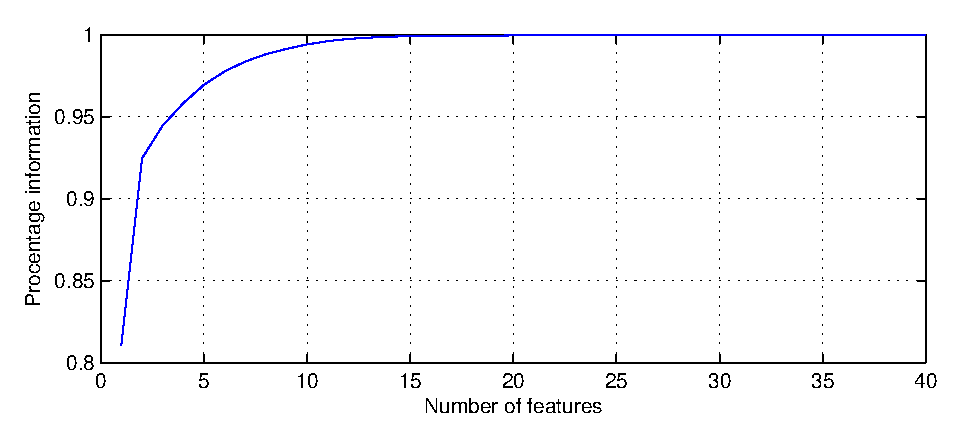
\includegraphics[width=\linewidth]{PCA_dist_var}
\caption{Cumulative distribution of variance (information) in dimensions sorted by highest eigenvalue}
\label{fig:PCA_dist_rap}
\end{figure} % DONE

	%!TEX root = Main.tex
\section*{Probabilistic Generative Models}
This part of the article, describes the Probabilistic Generative models (PGM).
The assumed probabilistic model for each class is a multivariate normal distribution. 
\begin{equation}
p(\mathbf{x}|C_k)=
\mathcal{N}(\mathbf{x};\mathbf{\mu}_k, \; \Sigma_k) 
\label{eq:gauss_dist} 
\end{equation}

\subsection*{Training}
In the training process the mean vector and covariance matrix of each class is estimated.

\begin{equation}
\bm{\mu}_k= \dfrac{1}{N} \sum_{j=1}^{N} \mathbf{x}_{kj} \\
\end{equation}

\begin{equation}
\bm{\Sigma}_k =
\dfrac{1}{N} 
\sum_{j=1}^{N} 
	(\mathbf{x}_{kj}-\bm{\mu}_k) 
	\cdot 
	(\mathbf{x}_{kj}-\bm{\mu}_k)
\end{equation}
The mean and covariance from the training is used to calculate the probability density for each class.
\begin{equation}
p(\mathbf{x}|C_k)=  
\dfrac{1}{(2\pi)^{D/2}} \dfrac{1}{\left|\mathbf{\Sigma} \right|^{1/2}} 
e^{
	-\dfrac{1}{2} 
	(\mathbf{x}-\bm{\mu}_k)^T 
	\bm{\Sigma}^{-1}
	(\mathbf{x}-\bm{\mu}_k) 
}
\end{equation}

The class prior is selected as an equal likelihood for each class. The probability of a given feature vector $ \mathbf{x} $ being part of a class $ C_k $ is given by.
\begin{equation}
p(C_k |\mathbf{x}) =
\dfrac{p(\mathbf{x}|C_k) p(C_k)}
{\sum_j p(\mathbf{x}|C_j) p(C_j)}
\end{equation}

\subsection*{Result}
The result of the probabilistic generative classifier is a total accuracy of 62.7, 58.1 and 57.2 \% respectively for one, two and ten digits.  % DONE?

	%!TEX root = Main.tex
\section*{Artificial Neural Networks}

The neural network model is a nonlinear function from a set of input variables $ \left\lbrace x_i \right\rbrace  $ transformed to a set of output variables $ \left\lbrace y_k \right\rbrace  $ controlled by the weight vector \textbf{w}, which is made of adjustable parameters.
The number of hidden units between the input and the output can be adjusted to the dataset.
This process is described in the following section.

The overall network function for a two layer neural network, takes the form
\begin{equation}
y_k(\mathbf{x},\mathbf{w}) = \sigma \left( \sum_{j=1}^{M} w_{kj}^{(2)} h\left( \sum_{i}^{D} w_{ji}^{(1)} x_i + w_{j0}^{(1)} \right) + w_{k0}^{(2)} \right) 
\label{eq:ANN_overall_rap}
\end{equation}
 
\begin{figure}[H]
	\centering
	\includegraphics[width=0.75\linewidth]{Figure5_1}
	\caption{Diagram of the two layer neural network. The nodes in the figure represents the input, hidden and output variable. The links between the nodes are the weight parameters. The figure is borrowed from \cite{bishop2007}} 
	\label{fig:ANN_fig_theory}
\end{figure}

\subsection*{Parametetric analysis}
The ANN was trained for the following number of hidden values: $ [10\ 20\ 50\ 100\ 200\ 300] $.
For each number of hidden values the training was done for $ 8 $ different values of $ \alpha $, uniformly space between 0 and 1.
for each value of alpha the training was tried 8 times and the mean and variance of the error was recorded. The results are visible below in Figure \ref{fig:ANN_error}.

\begin{figure}[H]
\centering
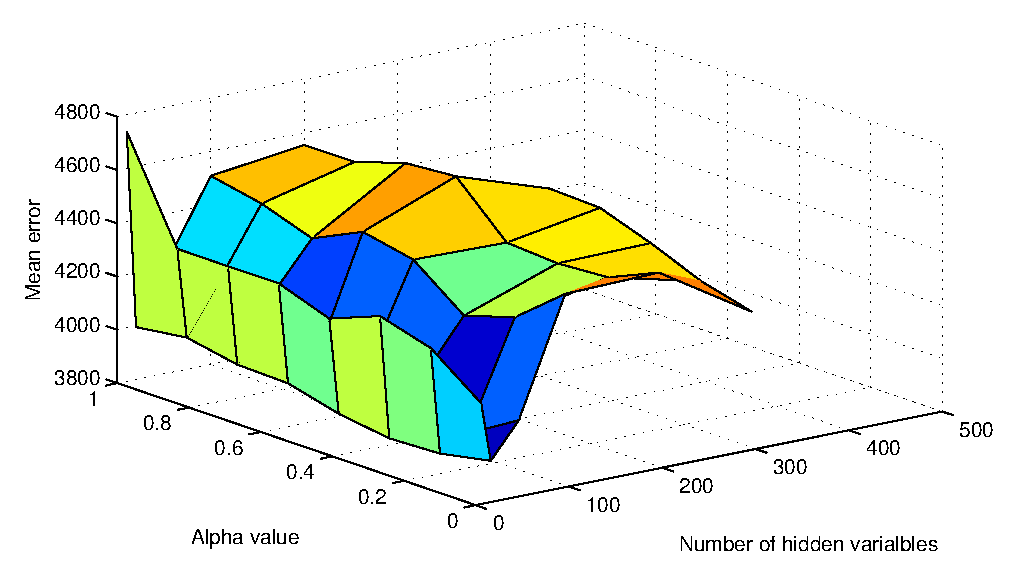
\includegraphics[width=\linewidth]{ANN_error}
\caption{Results of parametric analysis. Mean error displayed.}
\label{fig:ANN_error}
\end{figure}

The number of hidden units was found to be optimal at 30, with an $ \alpha $ of 0.30. This is used for all of the datasets.

\subsection*{Training}
In the training of the neural network for a multi-class classification problem the following error-function is minimized.
\begin{equation}
E(\mathbf{w}) = \dfrac{1}{2} \sum_{n=1}^{N}\| \mathbf{y}(\mathbf{x}_n,\mathbf{w})-\mathbf{t}_n \|^2+\lambda| \mathbf{w}^T \cdot \mathbf{w}|
\label{eq:ANN_error_rap}
\end{equation}

To do the actual trianing and parameteric analysis of the neural networks the free Netlab toolbax for matlab was used \cite{Netlab}

\subsection*{Results}
The result of the ANN is a total accuracy of 95.3, 93.1 and 89.4 \% respectively for one, two and ten digits. 
The overall accuracy of the ANN model is very good, and the model can be used as an reliable speaker recognition classifier.   

	%!TEX root = Main.tex
\section*{Gaussian Mixture Models}
Gaussian Mixture Models (GMM) is a way of finding and describing sub-populations in clusters of data points.
It is done by fitting a specified number of Gaussian distributions to a population of data points.
Each distribution is a component of the model. 
The individual data points are then arranged into clusters based on which model component is most likely given the observed data point.

The distributions of the mixture model are fitted to data by iteratively employing Expectation Maximization (EM).

\subsection*{The EM Algotrithm}
In EM a mixture model is iteratively updated by esitimating model parameters $\bm{\mu}_k $ (component means) and $ \bm{\Sigma}_k $ (component covariance matrix) based on current assignment of responability and then reassigning responability based on new model parameters, starting out with a random guess of $\bm{\mu}_k \text{ and } \bm{\Sigma}_k \text{ for } k=1..K$ 


\subsubsection*{Initialization:}
\begin{enumerate}
\item
Choose initial estimates for model parameters $ \mathbf{\pi}_{k}, \mathbf{\mu}_{k}, \mathbf{\Sigma}_{k} $.

\begin{itemize}

	\item
	$ k $ is the component number out of K.

	\item
	$ \pi_{k} $  is the weight of the \textit{k}th component.

	\item
	$ \mathbf{\mu}_{k}$ is the mean of the \textit{k}th component.

	\item
	$ \mathbf{\Sigma}_{k} $ is the covariance matrix of the \textit{k}th component.

	\end{itemize}


\item
Compute the initial log-likelihood og the model

\begin{equation} \label{eq:loglikeGMM}
\ln p\left(X | \mathbf{\mu}, \mathbf{\Sigma}, \pi\right) = 
\sum_{n=1}^{N} \ln \sum_{k=1}^{N} \pi_{k}\mathcal{N}(\mathbf{x}_{n}|\mathbf{\mu}_{k},\mathbf{\Sigma}_{k})
\end{equation}

\end{enumerate}

\subsubsection*{E-step:}
Calculate the probability of each point in each component in order to assing responsibility

\begin{equation}
\gamma_{nk} = 
\frac
{\pi_{k}\mathcal{N}(\mathbf{x}_{n}|\mathbf{\mu}_{k},\mathbf{\Sigma}_{k})}
{\sum_{j=1}^{K} \pi_{n}\mathcal{N}(\mathbf{x}_{n}|\mu_{j},\mathbf{\Sigma}_{j})}
\end{equation}

\subsubsection*{M-step:}
Estimate new guesses for $ \mathbf{\pi}_{k}, \mathbf{\mu}_{k}, \mathbf{\Sigma}_{k} $.

\begin{equation}
\mathbf{\mu}_{k}^{new} = 
\frac{1}{N_{k}}
\sum_{n=1}^{N} 
\gamma_{nk}
\mathbf{x}_{k}
\end{equation}

\begin{equation}
\mu_{k}^{new} = 
\frac{1}{N_{k}}
\sum_{n=1}^{N} 
\gamma_{nk}
(\mathbf{x}_{k} - \mathbf{\mu}_{k}^{new})
(\mathbf{x}_{k} - \mathbf{\mu}_{k}^{new})^{T}
\end{equation}

\begin{equation}
\pi_{k}^{new} =
\frac
{N_{k}}
{N}
\end{equation}

\subsubsection*{Convergence check:}

Recalculate log likelihood using Equation \ref{eq:loglikeGMM}.
If the log likelihood has not changed more than some predetermined threshold stop iteration.
Otherwise continue from E-step.

\paragraph*{Training}
GMM is a tyoe of unsupervised machine learning, and is a first hand not usefull in our project, but by training a GMM for each speaker based on the pre-classfied trainging set, you end up with a very effective model.


Then, for each speaker, a GMM is fitted to the respective speakers' training data, using MATLAB's Statistics Toolbox.

\paragraph*{Result}
 % DONE

	%!TEX root = Main.tex
\section*{Support Vector Machines}
In this section the soft margin support vector machine (SVM) is described. 
The SVM is a binary classifier, which is a problem with multi class. 
The solution for multiclass classification is using a one-vs.-one setup.
The decision function for a standard SVM for a test point $ x_{new} $ is given by
\begin{equation}
t_{new} = \mathtt{sign}(\mathbf{w}^T \mathbf{x}_{new} +b)
\label{eq:SVM_lin}
\end{equation}

\subsection*{Training}
The parameter vector $ \mathbf{w} $ is found by maximizing the margin or minimizing the length of the parameter vector, because of the inverse relationship $ \gamma = \frac{1}{\|\mathbf{w}\|} $.
In the training process of a soft margin SVM, the following expression is minimized. 
\begin{align}
\mathbf{w}^* = 
\mathtt{argmin}_\mathbf{w} \frac{1}{2} \mathbf{w}^T \mathbf{w}+C \sum_{n=1}^{N} \xi_n,\\ \mathtt{w.r.t.} \qquad t_n(\mathbf{w}^T \mathbf{x}_n + b) \geq 1-\xi_n
\end{align} 
The influence of each training point in the decision boundary is proportional to $ \alpha_n $.
After the training process, the classification can be done by using the following expression, where $ \mathbf{x}_n $  are the support-vectors, and $ \alpha_n $ is their weights.
\begin{equation}
t_{new} = 
\mathtt{sign}\left( \sum_{n=1}^{N} \alpha_n t_n k(\mathbf{x}_n,\mathbf{x}_{new}) +b  \right)
\end{equation}
with $ k = \mathtt{exp}(-\gamma \|\mathbf{x}^T_n - \mathbf{x}_{new} \|^2 ) $, which is the Gaussian kernel.

\subsection*{Results}
The result was obtained by using a Gaussian kernel, and the classification accuracy was found to be 73.7 \% for the one digit dataset after training on the training set and afterwards classifying the test set.

\section*{Discussion}
This section contains a brief discussion of the results of the five different classification methods which have been used throughout this project. The resulting accuracy is shown on table \ref{table:result}.

\begin{table}[h]
\begin{tabular}{@{}l|lll@{}}
\toprule
Model 		   		   & One digit            & Two digits  & Ten digits   \\ \midrule
ANN                    & 95.3 \%                & 93.1 \%   & 89.4 \% \\
GMM                    & 94.6 \%                & 91.2 \%   & 89.1 \% \\
SVM                    & 73.7 \%                & - 	    & -       \\ 
PGM                    & 62.7 \% 				& 58.1 \%   & 57.2 \% \\
Linear                 & 55.9 \% 				& 51.2 \%   & 50.6 \%

\end{tabular}
\caption{The table shows the overall accuracy of classification for the model used in this project. }
\label{table:result}
\end{table}

In this project the speaker base only contain three people and are therefore fairly limited. 
Some of the models that was used to classify the data may not work with different speakers or a large group of speakers.
To make the models more robust are large base of speakers is needed.
For some of the models three speakers base is already at the limited of the computer power and time available.\\

A way to make the models more robust is the usage of a universal background model.
The UBM is described in \cite{Springer:36}.\\

The lowest classification accuracy is found in the linear models, which was expected because of the simplicity of the model.
The dataset has a lot of dimensions and overlapping, and therefore too complex for a linear decision boundary.
The second lowest classification accuracy is found in the probabilistic generative model. 
The PGM is also too simple a model to handle the dataset, but still more complex than the linear model, which is expressed in the accuracy.
One of the problems with PGM is that numbers of independent variable that have to be determined for each class scale with the number of dimensions.\\

The middle accuracy model is the support vector machine.
The training phase needs to be iterated a large number of times, and therefore takes a considerable time to do. 
The result of the smallest dataset isn't that accurate so it was not worth applying the model on the other two datasets.\\

The model with the second highest classification accuracy is the Gaussian mixture model.
The model have a overall accuracy close to ANN, and are working well as a classifier for speaker recognition. 
The reason for the good result can be that the GMM have more than one Gaussian to describe each class.
The training phase of GMM was computational load heavy, but the classification didn't demand so much.\\

The model that have the highest classification accuracy of speaker recognition is the artificial neural network.
The model was found to be very demanding regarding the computational load during the training phase. 
This is because the ANN doesn't have a single minimum, and therefore the training needs to be iterated a large number of times. 






%!TEX root = Main.tex
\section*{Conclusion}
In this project five classification methods were used for speaker recognition.
The dataset consisted of three different speakers, saying the digits 0-9, divided onto three datasets.
One with one digits, one with two digigts and one with ten digits expressed.\\

The different methods was implemented through MATLAB and compared using the confusion matrix and the overall accuracy.
The result is that we can determine who is speaking it is down to 95.3 \% for one digit and 89.4 \% for ten digits.
The model that gave the best result was the Artificial Neaural Networks with Gaussian Mixture Models as a close contender.

  


\bibliographystyle{ieeetr}
\renewcommand{\bibname}{2 Reference Document}
\addcontentsline{toc}{chapter}{2 Reference Document}
\bibliography{Appendix/10731@post.au.dk-RefList}



\end{document}
